\section{The Plug-In}
Introduction to the chapter.
	What elements are there in this chapter?		
		EasyInsert
		Dialogs
		Settings		
		Device tab
		Geo tab
		Delete tab


\subsection{Dialog Windows}
Something about what dialogs does, and why we use em.

The dialogs of EasyInsert has been implemented in it's own class dialog.hpp, i.e. a subclass of QDialog, see figure~\ref{fig:subClassQWidget} for an example of a Qt subclass. This was done to keep it independent and self-contained from the rest of the plug-in. Since the dialog class is a subclass of QDialog, the position of the dialog window (opposed to a normal QDialog object) is always centred to the main application, even though a parent is passed as a parameter.

The constructor for the dialog class is very simple, see figure~\ref{fig:dialogConstructor}. A constructor with no WorkCell parameter is also available, though a name and parent must always be given to the constructor. 

\begin{figure}[h]
\centering
\lstset{language=C++} 
\begin{lstlisting}[frame=single]  
dialog::dialog(rw::models::WorkCell::Ptr wc, QString dialog, QWidget *parent)
    : QDialog(parent)
{
    _workCell = wc;
    mainLayout = new QVBoxLayout();
    setWindowTitle(dialog);
}			 
\end{lstlisting}
\caption{The dialog class constructor. A WorkCell pointer to a RW instance is passed along as a parameter. The QString parameter is the name of the dialog box and the QWidget is a pointer to the parent widget }
\label{fig:dialogConstructor} 	
\end{figure}

The dialog class is fairly simple to use and extend. A dialog is made of blocks in a vertical layout of QWidget's, i.e. a dialog instance is a composite widget containing composite widgets. Figure~\ref{fig:dialogclassblocks} shows a dialog window with four blocks initialised. These blocks are just member functions of the dialog class which returns their parent widget. So to create a dialog window as shown on figure~\ref{fig:dialogclassblocks}, a dialog instance should be constructed (in this case with a WorkCell pointer) and then simply add the widgets to the layout with the utility member function addToDialog(). See figure~\ref{fig:dialogWindowCode} which shows how to use the dialog class to make the dialog window as shown on figure~\ref{fig:dialogclassblocks}. 

\begin{figure}[h]
	\centering
	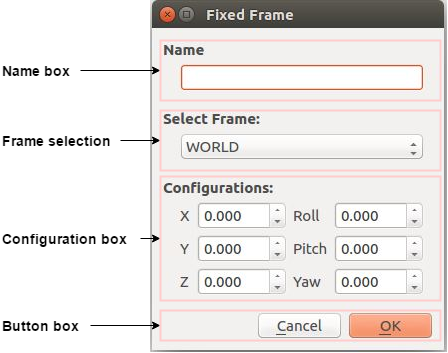
\includegraphics[scale=0.55]{Figures/dialogclassblocks.png}
	\caption{This figure shows a dialog window of adding a fixed frame to a WorkCell containing various widgets relevant to the action. }
	\label{fig:dialogclassblocks}
\end{figure}

\begin{figure}[h]
\centering
\lstset{language=C++} 
\begin{lstlisting}[frame=single]  
QString st = "Fixed Frame";
rw::models::WorkCell::Ptr wc = getRobWorkStudio()->getWorkCell();
_geometriDialog = new dialog(wc,st,this);
_geometriDialog->addToDialog(_geometriDialog->createNameBox());
_geometriDialog->addToDialog(_geometriDialog->createFrameSelection());
_geometriDialog->addToDialog(_geometriDialog->createConfigurationBox());
_geometriDialog->addToDialog(_geometriDialog->createButtonBox());		 
\end{lstlisting}
\caption{A sample code to illustrate how to construct the dialog window from figure~\ref{fig:dialogclassblocks}.}
\label{fig:dialogWindowCode} 	
\end{figure}







